\section{État de l'art}%{{{

Rq Sarah 01/03

\begin{itemize}
\item
  3.2 on ne peut être que partiellement sensible au flot dans ce type
  d'analyse non ?
\item
  dans les techniques classiques, tu as aussi le software model checking
  et le SMT solving
\item
  remarque générale sur ce chapitre : pourquoi ne pas parler seulement
  du C puisque tu ne traites ensuite que de cela ?
\end{itemize}


\begin{itemize}
\item difficultés : récursion

\item
  types : citer H98\cite{haskell98}, perl \cite{perlCamelBook}, DAOC\cite{DAOC}
  \& RWH\cite{rwh}?
\item
  Analyse de flot :
Ce que nous voulons vérifier peut être vue comme une propriété de flot. Un tour
d'horizon des problèmes et techniques existantes peut être trouvé
dans~\cite{sm-jsac03}.

\item Divers : Taint sequences \cite{mdv10}, % MLP/Mounier

L'interprétation abstraite a été utilisée pour analyser le flot de données entre
objets~\cite{liang2012taint}.

\end{itemize}

L'analyse de taintage consiste à ajouter des étiquettes au données décrivant
leur provenance, de manière à ce que chaque accès dangereux soit vérifié à
l'exécution. Cela se marie bien avec les langages typés dynamiquement, comme le
montre l'exemple célèbre du mode «souillé» (\emph{tainted}) de
Perl~\cite{perlCamelBook}. Il est aussi possible, d'appliquer
cette technique à des langages compilés~\cite{clause-etal-issta07,oakland10}.
En revanche cela est plus délicat car l'environnement d'exécution n'est pas
autant contrôlé.

% TODO [E]: à préciser

\begin{itemize}
\item
Les pointeurs sur fonction rendent floue la limite qui est habituellement
présente entre instructions et données. En leur présence il est impossible de
faire une analyse de flot de contrôle indépendante du flot de données. Pour
pouvoir les traiter, il faut que le domaine abstrait en question soit assez
précis pour qu'un pointeur abstrait se concrétise en un ensemble réduit de
fonctions. Dans le cas où le domaine ne peut pas borner l'ensemble des fonctions
possibles et renvoie $\top$, l'analyse ne peut pas continuer.

\item
L'allocation dynamique de données, présente dans le langage C par le biais des
fonctions \texttt{malloc} et \texttt{free}, modifie le modèle mémoire
nécessaire. Sans celle-ci, l'ensemble des zones mémoire possibles peut être
décrit statiquement : ce sont les noms de variable. Ce qu'introduit
\texttt{malloc} au langage, c'est une zone mémoire qui n'a pas de nom, et sur
laquelle on n'a qu'un pointeur.

% TODO, bof + expand

\item
Le transtypage (\emph{casts}) entre entiers et pointeurs est particulièrement
délicat à traiter. Dans les modèles abstraits, les pointeurs sur données ou sur
fonctions n'ont pas de représentation numérique, seulement une représentation
symbolique. Même dans l'exécution concrète, la représentation numérique d'un
pointeur est lié à de nombreux choix faits par l'environnement d'exécution
(comme la randomisation de l'espace d'adressage) qui ne peuvent pas facilement
être modélisés.

\item
Les nombres flottants (types \texttt{float}, \texttt{double} et \texttt{long
double}) ont une sémantique particulière, et il n'est pas correct d'approcher
leur sémantique par une sémantique dans $ℝ$. Afin d'être correct, il faut
établir des domaines spécifiques au flottant, comme~\cite{floatpoly}. Un tour
d'horizon des difficultés liées aux flottants est effectué
dans~\cite{floatpitfalls}.

\end{itemize}

% TODO [E] setjmp/longjmp, unions

%}}}

\section{Évaluateur} % {{{

% --- Comparaison à C

Le langage C~\cite{KandR} est un langage impératif, conçu pour être un
«assembleur portable». Ses types de données et les opérations associées sont
donc naturellement très bas niveau.

Les types de données de C sont établis pour représenter les mots mémoire
manipulables par les processeurs : essentiellement des entiers et flottants de
plusieurs tailles. Les types composés correespondent à des zones de mémoire
contigües, homogènes (dans le cas des tableaux) ou hétérogènes (dans le cas des
structures).

Une des spécificités de C est qu'il expose au programmeur la notion de pointeur,
c'est-à-dire des variables qui représentent directement une adresse en mémoire.
Les pointeurs peuvent être typés (on garde une indication sur le type de l'objet
stocké à cette adresse) ou non typés.

Le système de types rudimentaire de C ne permet pas d'avoir beaucoup de
garanties sur la sûreté du programme. En effet, aucune vérification n'est
effectuée en dehors de celles faites par le programmeur.

Le but ici est d'établir un langage plus simple mais qui permettra de raisonner
sur une certaine classe de programmes C.

% TODO mettre ailleurs ?

\begin{itemize}
\item Exp-AddrOf sur toutes les lv
\item figures gramdef : singulier ou pluriel?
\end{itemize}

Limitations :

\begin{itemize}
\item tableaux de taille dynamique ?
\end{itemize}

\subsection*{Extrait PLAS}



% }}}

\section{Typage}%{{{

\begin{itemize}
\item ordre des sections
\item versions $Γ ⊢ i$ des propriétés
\item preuve de progres : état mémoire : doublet/triplet
\item définir les opérations d'ajout/remplacement sur les contextes de typage
\item 2 pointeurs peuvent etre égaux sans comparer les valeurs pointées
\item extension de contextes : :: ou , ?
\end{itemize}

\subsection*{Fonctions}

\begin{itemize}
\item
  page 50 règle CALL une remarque disant que cette règle doit être
  utilisée avec une autre qui va typer le corps de la fonction (mettre
  la ref) parce que sinon ça surprend
\item
  5.5 le fait de choisir une unique variable R t'oblige à ajouter une
  opération de suppression du R de la fonction appelante factice.
  Pourquoi ne pas générer des variables fraîches à partir du nom de la
  fonction + un identifiant unique ?
\item
  lemme 5.1 cas fonction, à quoi ça sert d'introduire la notation t'
  alors qu'il n'apparaît pas dans une règle ?
\end{itemize}

\subsection*{Rq}
(passe Sarah 17/01)

\begin{itemize}
\item
  5.3 left-values la règle LV-VAR suppose que x n'apparaît qu'une fois
  dans $\Gamma$ ou alors toujours accompagné du même type
\item
  p53 le terme de dérivation (première phrase de la preuve) n'a jamais
  été expliqué ?
\item
  lemme 5.1 constantes. Il faut expliquer à quel ensemble n et f
  appartiennent
\item
  lemme 5.2 même remarque que 5.1 concernant n et f (plus confusion f
  float et f fonction)
\item
  lemme 5.3 ça ne marche que si une variable n'apparaît qu'une fois dans
  le contexte ou avec toujours le même type (cf rem ci-dessous sur 5.3)
\item
  il manque les preuves de 5.3 et 5.4
\item
  théormèe 5.2 rappeler où a été défini l'évaluation d'une expression et
  dans quel cas elle produit des valeurs
\end{itemize}%}}}

\section{Qualificateurs}%{{{

\begin{itemize}
\item appliquer taint sur des sous-valeurs?
\item vTaint doit se propager aux accès de champ
\item étendre l'état mémoire aux variables utilisateur
\end{itemize}

(passe Sarah)

\begin{itemize}
\item
  6.1.1 français dans «qui représente qui contrôle sa valeur»
\item
  6.1.1 mettre une ref sur la description du noyau linux
\item
  la traduction de taintage par teintage est incorrecte (et des fois du
  garde la même orthographe que celle anglaise avec le `a') La
  traduction de tainted c'est plutôt sali, pollué. Tu peux aussi garder
  le terme anglais et le mettre en italique
\item
  j'ai arrêté de lire à partir de 6.2 parce que le texte n'est pas
  vraiment clair
\end{itemize}

Sarah 13/02

\begin{itemize}
\item
  expliquer pourquoi on a besoin d'étendre l'expressivité de C\_ML
  (rappeler le contexte des pointeurs usr et kernel et dire que ce sont
  les ptrs maitrises par le usr qui sont souillés)
\item
  typo intro systme
\item
  6.1 phrase «tout d'abord\ldots{}» pas très français non ?
\item
  5.1 étape «ensuite» à quoi correspond le phi ?
\item
  figure 6.1 ça serait plus propre de tout remettre et surligner/colorer
  les nouveautés (à expliquer dans le texte)
\item
  6.2 pourquoi ne pas nommer cette extension de C\_ML
\item
  3ème parag 6.3 choisir entre «qui représente» et «qui contrôle»
\item
  idem figure 6.2 ça serait plus clair de remettre tout
\item
  je me demande si ça ne serait pas plus clair de présenter d'abord
  l'extension des types ptr à KERNEL et USR et ensuite d'expliquer que
  ce qu'on cherche c'est de voir quelles expressions/valeurs sont
  TAINTED (donc à mettre après)
\end{itemize}


% le cimetière des règles

%\begin{mathpar}
%\irule{Taint-Erase}
  %{ }
  %{ \mmi{m}{\iTaint{x}}{m}{\iPass} }
%\end{mathpar}

%\begin{mathpar}
%\irule{Taint-Write-Old}
  %{ }
  %{ \mmi{m}{\iTaint{x}}{m[x ← \vTainted{m[x]}]}{\iPass} }
%\end{mathpar}

%\begin{mathpar}
%\irule{Taint-Write}
  %{ }
  %{ \mmi{m}{\iTaint{φ}}{m[φ ← \vTainted{m[φ]}]}{\iPass} }
%\end{mathpar}

\section*{Extrait PLAS}

The main distinctiveness is that instead of having a plain pointer type
$t~*$, our one is decorated with a type qualifier $q$. This annotation expresses
who controls the value of the pointer. If the kernel controls the value of the
pointer, then it cannot be abused. On the other hand, one has to be careful
with user-controlled pointers, because the caller can abuse the kernel and
access reserved memory. The only safe case when dereferencing such a pointer is
if its value is outside the kernel's memory.

In order to avoid dangerous cases, we have to dynamically check that the
destination of every user-controlled pointer is in userspace. Kernel pointers
(that is to say, kernel-controlled pointers) can be dereferenced without further
check, but user pointers have to be manipulated with a restricted interface that
will check whether their destination is in userspace.

As mentioned before, this is done using the following constructs:%
{\small
\begin{mathpar}
    \disprule{GetU}

    \disprule{PutU}
\end{mathpar}}%
To add qualifiers to a type system, the rules of interest are those that
manipulate pointers: dereferencing, pointer arithmetic and referencing (taking
the address of a left-value).

Dereferencing the easiest one ; our goal is to authorize dereferencing only
\qKernel pointers:

{\small \[ \disprule{Lv-Deref} \]}%

Pointer arithmetic can be done inside a \qUser or \qKernel memory zone. There is
no concern of jumping from userspace to kernelspace, because pointer arithmetic
is checked at runtime: if these operators overflow or are applied to a bad
pointer (such as a pointer to an integer field), $\serr{ptr}$ is raised.

{\small \[ \disprule{Ptr-Arith} \]}%

The reference case is trickier because a type qualifier has to be synthesized.
Because it is created on the kernel stack, it has a \qKernel qualifier in all
cases:
{\small \[
  \disprule{Addr}
\]}%

The $\eTaint{\cdot}$ operator turns a \qUser pointer into a \qKernel pointer.
It is an important rule, because it is the only source of \qUser pointers in the
type system.

The return value of a function is emulated with a virtual left-value $\vRet$.%
{\small \begin{mathpar}
  \disprule{Return}

  \disprule{Fun}
\end{mathpar}}%%}}}

\section{Implem}%{{{

\subsection{Prétraitement}

\ctonewspeak{} travaillant uniquement sur du code prétraité (dans directives de
préprocesseur), la première étape consiste donc à faire passer le code par \cpp:
les macros sont développées, les constantes remplacées par leurs valeurs, les
commentaires supprimés, les fichiers d'en-tête inclus, etc.

\subsection{Compilation (levée des ambigüités)}

Cette passe est réalisée par l'utilitaire \ctonewspeak{}. L'essentiel de la
compilation consiste à mettre à plat les définition de types, et \subsection{Annotations}

\newspeak{} a de nombreux avantages, mais pour une analyse par typage il est
trop bas niveau. Par exemple, dans le code suivant

\begin{Verbatim}[commandchars=\\\{\}]
\PY{k}{struct} \PY{n}{s} \PY{p}{\PYZob{}}
    \PY{k+kt}{int} \PY{n}{a}\PY{p}{;}
    \PY{k+kt}{int} \PY{n}{b}\PY{p}{;}
\PY{p}{\PYZcb{}}\PY{p}{;}

\PY{k+kt}{int} \PY{n+nf}{main}\PY{p}{(}\PY{k+kt}{void}\PY{p}{)}
\PY{p}{\PYZob{}}
    \PY{k}{struct} \PY{n}{s} \PY{n}{x}\PY{p}{;}
    \PY{k+kt}{int} \PY{n}{y}\PY{p}{[}\PY{l+m+mi}{10}\PY{p}{]}\PY{p}{;}
    \PY{n}{x}\PY{p}{.}\PY{n}{b} \PY{o}{=} \PY{l+m+mi}{1}\PY{p}{;}
    \PY{n}{y}\PY{p}{[}\PY{l+m+mi}{1}\PY{p}{]} \PY{o}{=} \PY{l+m+mi}{1}\PY{p}{;}
    \PY{k}{return} \PY{l+m+mi}{0}\PY{p}{;}
\PY{p}{\PYZcb{}}
\end{Verbatim}


\subsection{Implantation de l'algorithme de typage}

On prend l'exemple d'un lambda-calcul simplement typé avec entiers, flottants et
couples (figure~\ref{fig:stlc}).

\begin{figure}

\gramlr{Termes}{
\begin{align*}
  t \gramisa & x              & \textrm{Variable} \\
    \gramor  & λ x . t        & \textrm{Abstraction} \\
    \gramor  & t              & \textrm{Application} \\
    \gramor  & n              & \textrm{Entier} \\
    \gramor  & f              & \textrm{Flottant} \\
    \gramor  & (t, t)         & \textrm{Couple} \\
    \gramor  & \textrm{fst}~t & \textrm{Projection gauche} \\
    \gramor  & \textrm{snd}~t & \textrm{Projection droite}
\end{align*}
}

\gramlr{Types}{
\begin{align*}
  τ \gramisa &  \tInt          & \textrm{Entier}\\
    \gramor  &  \tFloat        & \textrm{Flottant}\\
    \gramor  & τ \rightarrow τ & \textrm{Fonction} \\
    \gramor  & τ \times τ      & \textrm{Produit}
\end{align*}
}

\gramlr{Contextes}{
\begin{align*}
  Γ \gramisa & ε     & \textrm{Contexte vide}\\
    \gramor  & Γ,x:τ & \textrm{Extension}
\end{align*}
}

\gramlr{Règles}{
\begin{mathpar}
\irule{Int}{ }{Γ⊢n:\tInt}
\and
\irule{Float}{ }{Γ⊢f:\tFloat}
\and
\irule{Var}{x:τ∈Γ}{Γ⊢x:τ}
\and
\irule{App}{Γ⊢f:τ_1 \rightarrow τ_2 \\ Γ ⊢ x : τ_1}{Γ ⊢ f x : τ_2}
\and
\irule{Abs}{Γ,x:τ_1⊢ y : τ_2}{Γ⊢ λx.y:τ_1 \rightarrow τ_2}
\and
\irule{Proj-g}{Γ⊢x:τ_1\times τ_2}{Γ⊢\textrm{fst}~x:τ_1}
\and
\irule{Proj-d}{Γ⊢x:τ_1\times τ_2}{Γ⊢\textrm{snd}~x:τ_2}
\and
\irule{Tup}{Γ⊢x:τ_1 \\ Γ⊢y:τ_2}{Γ⊢(x,y):τ_1 \times τ_2}
\end{mathpar}
}


\caption{Lambda calcul simplement typé avec entiers, flottants et couples}
\label{fig:stlc}

\end{figure}

Prenons l'exemple de la fonction suivante\footnote{ On suppose que \texttt{plus}
est une fonction de l'environnement global qui a pour type $\tInt \rightarrow
\tInt \rightarrow \tInt$.} :

\[
f = λx.λy. \textrm{plus} (\textrm{plus} (\textrm{fst} x) (\textrm{snd} x)) y
\]

Soit en syntaxe ML :

\begin{Verbatim}
let f x y =
  plus
    (plus
      (fst x)
      (snd x)
    )
    y
\end{Verbatim}

Puisque \texttt{fst} et \texttt{snd} sont appliqués à \texttt{x}, ce doit être
un tuple. En outre on additionne ces deux composantes ensemble, donc elles
doivent être de type \tInt (et le résultat aussi). Par le même argument,
\texttt{y} doit aussi être de type \tInt. En conclusion, \texttt{x} est de type
$\tInt × \tInt$ et \texttt{y} de type $\tInt$, donc f est de type $\tInt × \tInt
→ \tInt → \tInt$.

Pour implanter cette analyse, on peut remarquer qu'étant donné la forme d'un
terme, on peut savoir quelle règle de typage a été utilisée en dernier. Il est
ainsi possible de «remonter» l'arbre d'inférence afin de savoir quelles règles
ont été employées (figure~\ref{fig:inftree-rules})\footnote{Par souci de clarté,
les prémisses des applications de \textsc{(Var)} ne sont pas notées.}. Pour le
moment, on ne connait pas les types.

\begin{figure} % {{{ Fig règles
\def\disptypeR#1#2{:#1}

\def\gammaXY{\ensuremath{Γ_2}}
\def\gammaX{\ensuremath{Γ_1}}
\def\gammaOneDef{\ensuremath{Γ^0, x\disptypeL{\tInt \times \tInt}, y\disptypeL{\tInt}}}
\def\gammaTwoDef{\ensuremath{Γ^0, x\disptypeL{\tInt \times \tInt}}}
\def\termFst#1{\ensuremath{\textrm{fst}~x}}
\def\termSnd#1{\ensuremath{\textrm{snd}~x}}
\def\fstx{\termFst{x}}
\def\sndx{\termSnd{x}}
\begin{mathpar}
\irule
  {Abs}
  {
    \irule
      {Abs}
      {
        \inferrule*[right=(App)]
          {
            \inferrule*[right=(Var), rightskip=4em]
              { }
              {\gammaXY ⊢ y
              \disptypeR{\tInt}
              }
            \\
            \inferrule*[right=(App),vdots=4em,leftskip=5em,rightskip=5em]
              {
                \inferrule*[right=(Var), leftskip=3em, rightskip=7em]
                  { }
                  {\gammaXY ⊢ \textrm{plus}
                  \disptypeR{\tInt \rightarrow \tInt \rightarrow \tInt}
                  }
                \\
                \inferrule*[right=(App),vdots=3em,leftskip=7em,rightskip=3em]
                  {
                    \inferrule*[right=(App), vdots=4em, rightskip=5em]
                      {
                        \inferrule*[right=(Var), rightskip=5em]
                          { }
                          {\gammaXY ⊢ \textrm{plus}
                          \disptypeR{\tInt \rightarrow \tInt \rightarrow \tInt}
                          }
                        \\
                        \inferrule*[right=(Proj-G), vdots=3em, leftskip=5em]
                          {
                            \irule
                              {Var}
                              { }
                              {\gammaXY ⊢ x
                              \disptypeR{\tInt \times \tInt}
                              }
                          }
                          {\gammaXY ⊢ \fstx
                          \disptypeR{\tInt}
                          }
                      }
                      {\gammaXY ⊢ \textrm{plus} (\fstx)
                      \disptypeR{\tInt \rightarrow \tInt}
                      }
                    \\
                    \inferrule*[right=(Proj-D), leftskip=5em, rightskip=4em]
                      {
                        \irule
                          {Var}
                          { }
                          {\gammaXY ⊢ x
                          \disptypeR{\tInt \times \tInt}
                          }
                      }
                      {\gammaXY ⊢ \sndx
                      \disptypeR{\tInt}
                      }
                  }
                  {\gammaXY ⊢ \textrm{plus} (\fstx) (\sndx)
                  \disptypeR{\tInt}
                  }
              }
              {\gammaXY ⊢ \textrm{plus} (\textrm{plus} (\fstx) (\sndx))
              \disptypeR{\tInt \rightarrow \tInt}
              }
          }
          {\gammaXY ⊢ \textrm{plus} (\textrm{plus} (\fstx) (\sndx)) y
          \disptypeR{\tInt}
          }
      }
      {\gammaX ⊢ λy. \textrm{plus} (\textrm{plus} (\fstx) (\sndx)) y
      \disptypeR{\tInt \rightarrow \tInt}
      }
  }
  {Γ_0 ⊢ λx.λy. \textrm{plus} (\textrm{plus} (\fstx) (\sndx)) y
  \disptypeR{\tInt \times \tInt \rightarrow \tInt \rightarrow \tInt}
  }
\end{mathpar}

\[\gammaX = \gammaTwoDef \qquad \gammaXY = \gammaOneDef\]


\caption{Arbre d'inférence : règles à utiliser}
\label{fig:inftree-rules}
\end{figure} % }}}

Une fois à cette étape, on peut donner un nom à chaque type inconnu : $t_1, t_2,
\ldots$. L'utilisation qui en est faite permet de générer un ensemble de
contraintes d'unification (figure~\ref{fig:stlc-const}).

Le symbole $?$ qui apparait dans les règles correspond à «n'importe quel
type», dans le sens où l'unification avec ce symbole est toujours possible.

\begin{figure} % {{{
  \def\stlcConst#1#2{
  \fbox{
    \begin{tabular}{m{3.5cm}||c}
      \raggedleft \fbox{\raggedleft \ensuremath{#1}} & \fbox{\ensuremath{#2}}
    \end{tabular}
  }
  }
  \centering
  \begin{tabular}{m{4cm}||lm{4cm}||l}
    \raggedleft
    $
    \irule{Var}
      { (x, t_x) ∈ Γ }
      { Γ ⊢ x : t_1 }
    $
    &
    $
      t_1 = t_x
    $
    &
    \raggedleft
    $
    \irule{Abs}
      { Γ, (x:t_x) ⊢     e : t_2 }
      { Γ          ⊢ λx. e : t_1 }
    $
    &
    $
      t_1 = t_x → t_2
    $
    \\
    \multicolumn{4}{c}{} \\
    \raggedleft
    $
    \irule{App}
      { Γ ⊢ e_1 : t_1
     \\ Γ ⊢ e_2 : t_2
      }
      { Γ ⊢ e_1~e_2 : t_3 }
    $
    &
    $
      t_1 = t_2 → t_3
    $
    &
    \raggedleft
    $
    \irule{Proj-G}
      { Γ ⊢ e : t_2 }
      { Γ ⊢ \termFst{e} : t_1 }
    $
    &
    $
      t_2 = t_1 × ?
    $
    \\
    \multicolumn{4}{c}{} \\
    \raggedleft
    $
    \irule{Proj-D}
      { Γ ⊢ e : t_2 }
      { Γ ⊢ \termSnd{e} : t_1 }
    $
    &
    $
      t_2 = ? × t_1
    $
    &
    \raggedleft
    $
    \irule{Tup}
       { Γ⊢e_1:t_1
      \\ Γ⊢e_2:t_2
      }{
        Γ⊢(e_1,e_2):t_3
      }
    $
    &
    $
    t_3 = t_1 \times t_2
    $
  \end{tabular}
\caption{Contraintes crées par les applications de règles}
\label{fig:stlc-const}
\end{figure} %}}}

\begin{figure}
\centering

\subbottom[Contraintes]{
  \label{fig:inf-constr-ex}
  \begin{minipage}{0.5\linewidth}
  \begin{align}
  t_1    &= t_x → t_2             \tag{Abs1} \\
  t_2    &= t_y → t_3             \tag{Abs2} \\
  t_5    &= t_4 → t_3             \tag{App1} \\
  t_4    &= t_y                   \tag{Var1} \\
  t_6    &= t_7 → t_5             \tag{App2} \\
  t_6    &= \tInt → \tInt → \tInt \tag{Var2} \\
  t_{10} &= t_8 → t_7             \tag{App3} \\
  t_9    &= ? × t_8               \tag{Proj-D1} \\
  t_9    &= t_x                   \tag{Var3} \\
  t_{11} &= t_{12} → t_{10}       \tag{App4} \\
  t_{11} &= \tInt → \tInt → \tInt \tag{Var4} \\
  t_{13} &= t_{12} × ?            \tag{Proj-G1} \\
  t_{13} &= t_x                   \tag{Var5}
  \end{align}
  \end{minipage}
}
\subbottom[Solution]{
  \label{fig:inf-sol-ex}
  \begin{minipage}{0.3\linewidth}
  \begin{align*}
  t_{1}  &= \tInt × \tInt → \tInt \\
  t_{2}  &= \tInt → \tInt         \\
  t_{3}  &= \tInt                 \\
  t_{4}  &= \tInt                 \\
  t_{5}  &= \tInt → \tInt         \\
  t_{6}  &= \tInt → \tInt → \tInt \\
  t_{7}  &= \tInt                 \\
  t_{8}  &= \tInt                 \\
  t_{9}  &= \tInt × \tInt         \\
  t_{10} &= \tInt → \tInt         \\
  t_{11} &= \tInt → \tInt → \tInt \\
  t_{12} &= \tInt                 \\
  t_{13} &= \tInt × \tInt         \\
  t_{x}  &= \tInt × \tInt         \\
  t_{y}  &= \tInt
  \end{align*}
  \end{minipage}
}

\caption{Contraintes d'égalité et solution obtenues à partir de la
figure~\ref{fig:inftree-rules}}

\end{figure}

% mal numéroté

On en déduit donc un ensemble de contraintes d'égalité
(figure~\ref{fig:inf-constr-ex}). La prochaine étape est de résoudre ce système.
D'après (App1) et (App2), $t_6 = t_7 → t_4 → t_3$ d'où par (Var2), $t_7 → t_4 →
t_3 = \tInt → \tInt → \tInt$. Le constructeur $→$ étant injectif, on a donc $t_3
= t_4 = t_7 = \tInt$. En procédant de même avec (App3) et (App4), on obtient
$t_8 = t_{12} = \tInt$. D'après (Proj-G1), (Var5), (Var3), et (Proj-D1) on a
$t_{12} × ? = t_{13} = t_{x} = t_9 = ? × t_{8}$, donc $t_x = t_{12} × t_8 =
\tInt × \tInt$. En remplaçant, on obtient tous les autres types
(figures~\ref{fig:inf-sol-ex}) et donc un arbre de typage complet
(figure~\ref{fig:inftree-full}).

\begin{figure} % {{{ Fig full tree
\def\disptypeR#1#2{:#2}

\def\gammaXY{\ensuremath{Γ_2}}
\def\gammaX{\ensuremath{Γ_1}}
\def\gammaOneDef{\ensuremath{Γ^0, x\disptypeL{\tInt \times \tInt}, y\disptypeL{\tInt}}}
\def\gammaTwoDef{\ensuremath{Γ^0, x\disptypeL{\tInt \times \tInt}}}
\def\termFst#1{\ensuremath{\textrm{fst}~x}}
\def\termSnd#1{\ensuremath{\textrm{snd}~x}}
\def\fstx{\termFst{x}}
\def\sndx{\termSnd{x}}
\begin{mathpar}
\irule
  {Abs}
  {
    \irule
      {Abs}
      {
        \inferrule*[right=(App)]
          {
            \inferrule*[right=(Var), rightskip=4em]
              { }
              {\gammaXY ⊢ y
              \disptypeR{\tInt}
              }
            \\
            \inferrule*[right=(App),vdots=4em,leftskip=5em,rightskip=5em]
              {
                \inferrule*[right=(Var), leftskip=3em, rightskip=7em]
                  { }
                  {\gammaXY ⊢ \textrm{plus}
                  \disptypeR{\tInt \rightarrow \tInt \rightarrow \tInt}
                  }
                \\
                \inferrule*[right=(App),vdots=3em,leftskip=7em,rightskip=3em]
                  {
                    \inferrule*[right=(App), vdots=4em, rightskip=5em]
                      {
                        \inferrule*[right=(Var), rightskip=5em]
                          { }
                          {\gammaXY ⊢ \textrm{plus}
                          \disptypeR{\tInt \rightarrow \tInt \rightarrow \tInt}
                          }
                        \\
                        \inferrule*[right=(Proj-G), vdots=3em, leftskip=5em]
                          {
                            \irule
                              {Var}
                              { }
                              {\gammaXY ⊢ x
                              \disptypeR{\tInt \times \tInt}
                              }
                          }
                          {\gammaXY ⊢ \fstx
                          \disptypeR{\tInt}
                          }
                      }
                      {\gammaXY ⊢ \textrm{plus} (\fstx)
                      \disptypeR{\tInt \rightarrow \tInt}
                      }
                    \\
                    \inferrule*[right=(Proj-D), leftskip=5em, rightskip=4em]
                      {
                        \irule
                          {Var}
                          { }
                          {\gammaXY ⊢ x
                          \disptypeR{\tInt \times \tInt}
                          }
                      }
                      {\gammaXY ⊢ \sndx
                      \disptypeR{\tInt}
                      }
                  }
                  {\gammaXY ⊢ \textrm{plus} (\fstx) (\sndx)
                  \disptypeR{\tInt}
                  }
              }
              {\gammaXY ⊢ \textrm{plus} (\textrm{plus} (\fstx) (\sndx))
              \disptypeR{\tInt \rightarrow \tInt}
              }
          }
          {\gammaXY ⊢ \textrm{plus} (\textrm{plus} (\fstx) (\sndx)) y
          \disptypeR{\tInt}
          }
      }
      {\gammaX ⊢ λy. \textrm{plus} (\textrm{plus} (\fstx) (\sndx)) y
      \disptypeR{\tInt \rightarrow \tInt}
      }
  }
  {Γ_0 ⊢ λx.λy. \textrm{plus} (\textrm{plus} (\fstx) (\sndx)) y
  \disptypeR{\tInt \times \tInt \rightarrow \tInt \rightarrow \tInt}
  }
\end{mathpar}

\[\gammaX = \gammaTwoDef \qquad \gammaXY = \gammaOneDef\]


\caption{Arbre d'inférence complet}
\label{fig:inftree-full}
\end{figure} % }}}


Pour effectuer une résolution de manière automatique, il faut une technique
d'unification. La manière la plus classique de procéder est due à
Robinson~\cite{robinson} et se déroule par substitution.


\clearpage

Pour résoudre ces contraintes, on commence par les simplifier : si $t_a
\rightarrow t_b = t_c \rightarrow t_d$, alors $t_a = t_c$ et $t_b = t_d$. De
même si $t_a \times t_b = t_c \times t_d$. Au contraire, si $t_a \rightarrow t_b
= t_c \times t_d$, il est impossible d'unifier les types et il faut abandonner
l'inférence de types. D'autre cas sont impossibles, par exemple $\tInt = t_1
\rightarrow t_2$ ou $\tInt = \tFloat$.

Une fois ces simplifications réalisées, les contraintes restantes sont d'une des
formes suivantes :

\begin{itemize}
\item
  $t_i = t_i$. Il n'y a rien à faire, cette contrainte peut être supprimée.
\item
  $t_i = t_j$ avec $i \ne j$ : toutes les occurrences de $t_j$ dans les autres
  contraintes peuvent être remplacées par $t_i$.
\item
  $t_i = x$ (ou $x = t_i$) où $x$ est un type concret : idem.
\end{itemize}

%C'est faux

\clearpage

\begin{figure} % fig:unifpartage {{{

  \subbottom{
  \label{fig:unifpartage:a}
  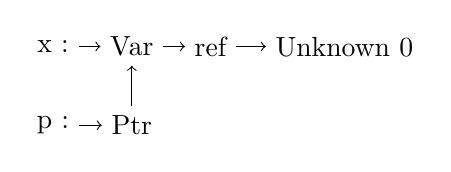
\begin{tikzpicture}
  \node               (var) {Var};
  \node[right of=var] (ref) {ref};
  \node[right of=ref, node distance=1.7cm] (u0) {Unknown 0};
  \node[below of=var] (ptr) {Ptr};
  \node[left of=var]  (x) {x :};
  \node[left of=ptr] (p) {p :};
  \draw[->] (x) -- (var);
  \draw[->] (p) -- (ptr);
  \draw[->] (ptr) -- (var);
  \draw[->] (var) -- (ref);
  \draw[->] (ref) -- (u0);
  \end{tikzpicture}
  }
  \subbottom{
  \label{fig:unifpartage:b}
  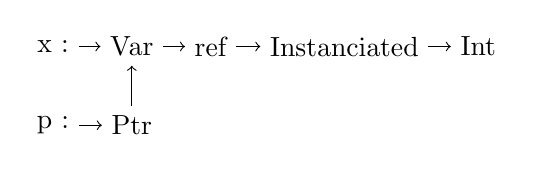
\begin{tikzpicture}
  \node               (var) {Var};
  \node[right of=var] (ref) {ref};
  \node[right of=ref, node distance=1.7cm] (u0) {Instanciated};
  \node[right of=u0, node distance=1.7cm] (ii) {Int};
  \node[below of=var] (ptr) {Ptr};
  \node[left of=var]  (x) {x :};
  \node[left of=ptr] (p) {p :};
  \draw[->] (x) -- (var);
  \draw[->] (p) -- (ptr);
  \draw[->] (ptr) -- (var);
  \draw[->] (var) -- (ref);
  \draw[->] (ref) -- (u0);
  \draw[->] (u0) -- (ii);
  \end{tikzpicture}
  }
  \subbottom{
  \label{fig:unifpartage:c}
  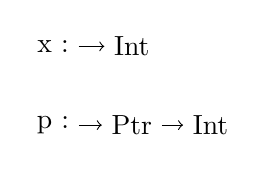
\begin{tikzpicture}
  \node               (var) {Int};
  \node[below of=var] (ptr) {Ptr};
  \node[left of=var]  (x) {x :};
  \node[left of=ptr] (p) {p :};
  \node[right of=ptr] (pi) {Int};
  \draw[->] (x) -- (var);
  \draw[->] (p) -- (ptr);
  \draw[->] (ptr) -- (pi);
  \end{tikzpicture}
  }

  \caption{Unification par partage}
  \label{fig:unifpartage}

\end{figure} % }}}

Plutôt que de modifier toutes les occurrences d'un type $t_i$, on va affecter à
$t_i$ la valeur du nouveau type.

L'implémentation de cet algorithme utilise le partage et les références
(figure~\ref{fig:unifpartage}).

D'abord \ref{fig:unifpartage:a}, ensuite \ref{fig:unifpartage:b}, et enfin
\ref{fig:unifpartage:c}.




\begin{figure} % fig:exunif:tpk {{{

  \insertcode{ex-unif-tpk.ml}

  \caption{Compilation d'un programme C -- après}
  \label{fig:exunif:tpk}
\end{figure} % }}}

Le programme C (figure~\ref{fig:exunif:c}) est compilé ainsi en Tyspeak
(figure~\ref{fig:exunif:tpk}).

\clearpage


The language described above, as well as a type inference algorithm, have been
implemented in OCaml as part of the Newspeak framework of program
analysis\cite{newspeak}. It is released under the GNU Lesser General Public
License, and is available on \texttt{http://penjili.org} (directory
\texttt{src/ptrtype} in the distribution). Our implementation consists of the
following steps.

but to analyze larger parts of the kernel, it may be
necessary to define a «maximal» configuration file (which is impossible
because of incompatibilities between some options).%}}}

\section{Étude de cas}%{{{

Le paramètre \texttt{data} provient de l'espace utilisateur via un appel
système. Un appelant malveillant peut se servir de cette fonction pour lire la
mémoire du noyau à travers le message d'erreur.

Le problème est modélisé de la façon suivante : on associe à chaque variable
\texttt{x} un type de données \texttt{t}, ce que l'on note \texttt{x:t}. En
plus des types présents dans le langage C, on ajoute une distinction
supplémentaire pour les pointeurs. D'une part, les pointeurs «noyau» (de type
\texttt{t~*}) sont créés en prenant l'adresse d'un objet présent dans le code
source. D'autre part, les pointeurs «utilisateurs» (leur type est noté
\texttt{t user*}) proviennent des interfaces avec l'espace utilisateur.

Il est sûr de déréférencer un pointeur noyau, mais pas un pointeur
utilisateur. L'opérateur \texttt{*} prend donc un \texttt{t *} en entrée
et produit un \texttt{t}.

Pour faire la vérification de type sur le code du programme, on a besoin de
quelques règles. Tout d'abord, les types suivent le flot de données.
C'est-à-dire que si on trouve dans le code \texttt{a = b}, \texttt{a} et
\texttt{b} doivent avoir un type compatible. Ensuite, le qualificateur
\texttt{user} est récursif : si on a un pointeur utilisateur sur une structure,
tous les champs pointeurs de la structure sont également utilisateur. Enfin, le
déréférencement s'applique aux pointeurs noyau seulement : si le code contient
l'expression \texttt{*x}, alors il existe un type \texttt{t} tel que
\texttt{x:t*} et \texttt{*x:t}.

Appliquons ces règles à l'exemple de la figure~X : on suppose que l'interface
avec l'espace utilisateur a été correctement annotée. Cela permet de déduire que
\texttt{data:void user*}. En appliquant la première règle à la ligne 6, on en
déduit que \texttt{info:struct drm\_radeon\_info user*} (comme en C, on peut
toujours convertir de et vers un pointeur sur \texttt{void}).

Pour déduire le type de \texttt{value\_ptr} dans la ligne 7, c'est la
deuxième règle qu'il faut appliquer : le champ \texttt{value} de
la structure est de type \texttt{uint32\_t~*} mais on y accède à travers
un pointeur utilisateur, donc \texttt{value\_ptr:uint32\_t user*}.

% faux

À la ligne 8, on peut appliquer la troisième règle : à cause du déréférencement,
on en déduit que \texttt{value\_ptr:t *}, ce qui est une contradiction puisque
d'après les lignes précédentes, \texttt{value\_ptr:uint32\_t user*}.

Si la ligne 3 était remplacée par l'appel à \texttt{copy\_from\_user}, il n'y
aurait pas d'erreur de typage car cette fonction peut accepter les arguments
\texttt{(uint32\_t~*, uint32\_t user*, size\_t)}.

Le principe de cette technique (associer des types aux valeurs puis restreindre
les opérations sur certains types) peut être repris. Par exemple, si on définit
un type «numéro de bloc» comme étant un nouvel alias de \texttt{int}, on peut
considérer que multiplier deux telles valeurs est une erreur.%}}}

\section{Conclusion}%{{{

\subsection{Future work}

We showed that type theory can be a useful tool for verifying the absence of
certain run-time properties. While adding static labels to variables seems to be
a crude approximation of reality, in some cases it has enough power to capture
real-world problems.

In this particular example, we work around C's lack of abstract types in order
to disallow dereference for a certain class of pointers, distinguished by
syntactic rules.

We defined an imperative language with an explicit stack, and described
operational semantics for it modelling that of the C programming language. It
includes a memory model that expresses the separation between user and kernel
spaces present in most operating systems. We added a type system that is sound
with respect to a property of isolation between this two memory spaces.

Finally, we demonstrate an implementation on this analysis on a bug that
affected the Linux kernel.

A first step towards making this analysis more practical is to demonstrate its
scalability by running it on larger fragments of the kernel.

There are also several places where we can improve significantly the
expressivity of our type system. For example, our current type system is only
monomorphic; but it would make sense to generalize free qualifier variables in
the type of global functions.%}}}

% Sarah 9/5

%chapeau de l'intro
%- manque de structures/liens entre les petits paragraphes.
%- il manque le plan de l'intro
%- incohérence entre tests exhaustifs et "on ne peut pas couvrir tout". En général, on dit que la taille actuelle des logiciels empêche l'exhaustivité des tests
%- dernier paragraphe pas clair : ça veut dire quoi restreindre la manière dont sont traitées les infos ? Tu peux peut-être détailler un peu plus puisque tu poses ici la problématique de ta thèse

%1.2
    %- tu pourrais ajouter un ex d'appel système en C pour expliquer le pb du déréférencement

%1.3
   %- typage fort et faible. On ne comprend pas la différence
   %- manquent des mots dans la dernière phrase de cette partie

%1.4
  %- pourquoi parler de C++ et Ada alors que tu ne vas traiter que le C ?

%1.5

%- il faudrait pour chaque front-end dire pourquoi ça n'est pas la solution retenue

%Pourquoi ne pas présenter informellement le cas d'étude dans l'intro
%pour montrer que de vrais bugs existent ?

% Emmanuel 6/5

  %Sur la première partie, je dirai que le point le plus important est de justifier ta proposition à la fin du ch
%+apitre 3,
   %et pour cela peut-être enlevé certains discussions préalables pour faire de 3.7 une vraie section complètemen
%+t argumentée.
  %Comme cela tu peux décrire CQual de manière neutre, puis dans la partie choix dire pourquoi avoir des types qu
%+alifiés te semble être la bonne démarche
    %avec un système de types plus simple et plus facile à exprimer.
